\documentclass[10pt,twocolumn,letterpaper]{article}

\usepackage{cvpr}
\usepackage{times}
\usepackage{epsfig}
\usepackage{graphicx}
\usepackage{amsmath}
\usepackage{amssymb}
\usepackage{booktabs}
\usepackage{array}
\usepackage{subcaption}
\usepackage{optidef}
\usepackage{xcolor}

% \usepackage{alphalph}
% \renewcommand\thesubfigure{\alphalph{\value{subfigure}}}


% Include other packages here, before hyperref.

% If you comment hyperref and then uncomment it, you should delete
% egpaper.aux before re-running latex.  (Or just hit 'q' on the first latex
% run, let it finish, and you should be clear).
\usepackage[pagebackref=true,breaklinks=true,letterpaper=true,colorlinks,bookmarks=false]{hyperref}

% \cvprfinalcopy % *** Uncomment this line for the final submission

\def\cvprPaperID{6485} % *** Enter the CVPR Paper ID here
\def\httilde{\mbox{\tt\raisebox{-.5ex}{\symbol{126}}}}

% Pages are numbered in submission mode, and unnumbered in camera-ready
\ifcvprfinal\pagestyle{empty}\fi

%commands and things
\renewcommand{\vec}[1]{\mathbf{#1}}
\newcommand{\Real}[1]{\mathbb{R}^{#1}}
\newcommand{\ReLU}{\texttt{ReLU}\,}
\newcommand{\ReLUBN}{\texttt{ReLU + BN}\,}
\newcommand{\moons}{\texttt{MOONS}\,}
\newcommand{\cifar}{\texttt{CIFAR-10}\,}
\newcommand{\SepConstraint}{\texttt{Sep-Cons}\,}
\newcommand{\SepUnit}{\texttt{Sep-U}\,}
\newcommand{\SepLayer}{\texttt{Sep-L}\,}
\newcommand{\SepPoint}{\texttt{Sep-P}\,}
\newcommand{\SepLayerBN}{\texttt{Sep-L-BN}\,}
\newcommand{\SepPointUnit}{\texttt{Sep-P+U}\,}
\newcommand{\layer}{\ell}
\newcommand\fuck[1]{\textcolor{red}{#1}}
\DeclareMathOperator*{\argmin}{arg\,min}


%%% theorem styles and stuff
\newtheorem{theorem}{Theorem}[section]
\newtheorem{corollary}{Corollary}[theorem]
\newtheorem{lemma}[theorem]{Lemma}
\newtheorem{remark}[theorem]{Remark}
\newtheorem{definition}{Definition}[section]


\title{Increasing separation in units for greater perforamnce an zero initialization}

\author{Riera-Molina C.\\
Universitat de Barcelona\\
Gran Via de les Corts Catalanes 585, Barcelona Spain, 08005\\
{\tt\small blauigris@gmail.com}
% For a paper whose authors are all at the same institution,
% omit the following lines up until the closing ``}''.
% Additional authors and addresses can be added with ``\and'',
% just like the second author.
% To save space, use either the email address or home page, not both
\and
Rey-Torres C.\\
Universitat de Barcelona\\
Gran Via de les Corts Catalanes 585, Barcelona Spain, 08005\\
{\tt\small camilorey@gmail.com}
}
\begin{document}
\maketitle

\section{Introduction}\label{sec:introduction}

% Párrafo introductorio
The success of Deep Learning has traditionally been linked to its ability to learn \emph{abstract representations} of data using function composition\cite{LeCun06atutorial}. These functions (i.e. the \emph{layers}) decompose and solve the problem in \emph{parts} \cite{resnetSubtree} profiting their feed-forward structure \cite{backprop}. However, the deeper the network, the more susceptible it becomes to issues affecting backpropagation as a learning strategy \cite{backprop} (e.g. the vanishing gradient problem, \cite{vanishing1,vanishing2} the exploding gradient \cite{exploding} and the dead unit problem \cite{leaky,whyreludie,whenneuronsfail}) . 
\\\\
% Problema general
There are \emph{essentially} two families of methods to address these issues: \emph{architectural modifications} to the network and input data \emph{manipulation}. Examples of architectural modifications include (1) layer-width increase as done in \cite{wideresnet,inceptionv1}; (2) feed-forward structure network modification, as done in ResNets \cite{resnet} or DenseNets \cite{densenet}; (3) unit based alterations (of the their non-linearity or activation) as done in \emph{leaky}-\ReLU \cite{leaky} or \texttt{PReLU} \cite{prelu}). Meanwhile, the most commonly used data manipulation technique is \emph{data normalization} techniques on the output of layers as done under \emph{batch normalization} \cite{batchnorm}.  
\\\\
For example, layer-width increases reduces the chance for \emph{useless} units (e.g. dead or \emph{redundant}) per layer. However, such measures increase the computational cost of the network and the dimensionality of the problem, hampering convergence \cite{cursedim} and taking a toll on speed. Meanwhile, modifying network connectivity may prove beneficial to tackle the vanishing gradient \cite{ladder,nin,highway}. This occurs however, at the expense of burdening designers with additional \emph{architectural} decisions (e.g. which connection to add or alter) taking a toll in parameter and hyper-parameter number as presented for example in \cite{densenet}. 
\\\\
In turn, unit activation modification intends to ensure non-zero gradient back-propagation by (1) modifying unit functions to avoid zero truncation as done in \cite{leaky}, \cite{prelu}, \cite{elu} or \cite{selu} (\ReLU modifications) or modifying unit output \cite{crelu}. With batch normalization \cite{batchnorm}, several drawbacks have been described in works like \cite{batchrenorm} and \cite{batchnormGradientExplosion}: decreased performance in testing due to non-matching statistical parameters between training and testing (e.g. mean value and variance or non-i.i.d. minibatches or small batch sizes \cite{batchrenorm}; and exploding gradients limiting the depth of the network \cite{batchnormGradientExplosion}.
\\\\
% Problema específico (Pregunta del paper)
Since existing methods require either computational expenditure and add arbitrary complexity to the architecture design, or simply entail limit network performance, we wonder whether we can train deeper networks without relying in any of those techniques. This imply using the minimum width possible, removing any additional connections or activations, and using no normalization. 
\\\\
We argue that those problems can be tackled at unit level, since they stem from the affine/dead unit problem. In this sense, we argue that 
affine unit \emph{downgrades} the unit to an redundant transform (since it can be carried out by the following unit), \emph{dead} units compromise the \emph{representative} ability of the network.
\\\\
While dead neurons have been traditionally accepted as a minor issue for DNN related phenomena, affine units are not usually seen as hazardous are also not devoid of caveats.
\\\\
% Solución propuesta (Respuesta a la pregunta)
We propose to achieve that by introducing a family of constraints which increase the separation performed by each of the units on the data. We demonstrate that doing so helps in avoiding trivial failure modes like dead or linear units. Additionaly, enables the use of zero initialization. The only added cost is an additional loss per layer and the inclusion of an additional hyperparameter. 
\\\\
% Estructura del paper
This paper is organized as follows: section \ref{sec:separability} motivates the importance of enforcing separation in the units), after that section presents the \ref{sec:constraint} the actual constraints that we impose on the network to do so. Section \ref{sec:experiments} provides with experimental interpretation of the effect of the constraints and finally section \ref{sec:conclusions} closes the paper with the main conclusions.

\begin{table*}[h!]
    \centering
\begin{tabular}{@{}llll@{}}
\toprule
Family                         & Method                                                             & Examples                                                                                                                                                                                                                                                   & Intended issues                                                                \\ \midrule
\multirow{3}{*}{Architectural} & Width increase                                                     & \begin{tabular}[c]{@{}l@{}}Wide \textbackslash{}texttt\{ResNet\} \textbackslash{}cite\{wideresnet\}\\ \textbackslash{}texttt\{Inception\} \textbackslash{}cite\{inceptionv1\}\end{tabular}                                                                 & \begin{tabular}[c]{@{}l@{}}Vanishing Gradient\\ Increase Depth\end{tabular}    \\
                               & \begin{tabular}[c]{@{}l@{}}Connection \\ modification\end{tabular} & \begin{tabular}[c]{@{}l@{}}\textbackslash{}texttt\{ResNet\} \textbackslash{}cite\{resnet\} \\ \textbackslash{}texttt\{DenseNet\} \textbackslash{}cite\{densenet\}\end{tabular}                                                                             & \begin{tabular}[c]{@{}l@{}}Vanishing Gradient\\ \\ Increase Depth\end{tabular} \\
                               & Unit Alteration                                                    & \begin{tabular}[c]{@{}l@{}}\textbackslash{}emph\{leaky\}-\textbackslash{}ReLU \textbackslash{}cite\{leaky\} \\ \textbackslash{}texttt\{PReLU\} \textbackslash{}cite\{prelu\}\\ \textbackslash{}texttt\{C-ReLU\} \textbackslash{}cite\{crelu\}\end{tabular} & \begin{tabular}[c]{@{}l@{}}Vanishing Gradient\\ Dead Neurons\end{tabular}      \\
Data Manipulation              & Modify layer output                                                & \textbackslash{}emph\{batch normalization\} \textbackslash{}cite\{batchnorm\}                                                                                                                                                                              & Exploding Gradient                                                             \\ \bottomrule
\end{tabular}
\end{table*}

\section{Neural networks and unit separability}\label{sec:separability}

A traditional so-called \emph{neural network} is composed of \emph{layers} whose input is the output of the previous \emph{layer} \ref{eq:layer}, which are composed of a set of arbitrary real-valued functions in $\mathbb{R}$ called \emph{units}\ref{eq:unit}. The units are commonly composed of an affine transform, parameterized by a vector of weights $\vec{w}$ and an scalar bias $b$, followed by a non-linear \emph{activation function} $\sigma : \mathbb{R}\rightarrow\mathbb{R}$. In the case of the \ReLU this activation function is consist in the truncation to zero of negative values.

\begin{equation}\label{eq:unit}
u(x; \vec{w}, b) = \sigma(\vec{w} \cdot \vec{x} + b)
\end{equation}
Given a collection $\vec{w}_1\ldots,\vec{w}_m\in\Real{m}$ of weight vectors and $b_1,\ldots,b_m\in\mathbb{R}$ a collection of bias, we simplify the notation via
\begin{equation}
    u_j(\vec{x}) = u(\vec{x};\vec{w}_j,b_j)
\end{equation}
for $j=1,\ldots,m$. Units can be linearly combined with canonical vectors of $\Real{M}$ to construct \emph{layer} functions $\layer:\Real{N}\rightarrow\Real{M}$ where $N$ is the layer \emph{dimension} and the number $M$ is the \emph{width} of the layer.

\begin{equation}\label{eq:layer}
\layer(\vec{x}) = \sum^M_{i=1} u_i(\vec{x}) \hat{\textbf{e}}_i
\end{equation}
on more plain terms, $\layer(\vec{x})$ is an $m$-tuple (a \emph{concatenation}) of the outputs of units $u_1,u_2,\ldots,u_m$.
\\\\
A DNN (a neural network) is a function $F:\Real{N_0}\rightarrow\mathbb{R}$ defined by a finite collection of size $L$ of layer functions which map the data points to the targets through function composition, by mapping a into a series of \emph{intermediate representations} \ref{eq:network}. \cite{ramachandranEtAl2017SearchingForActivationFunctions,eswaranSingh2015SomeTheoremsForFFNN}.

\begin{equation}\label{eq:network}
F(x) = \layer_D \cdot \layer_{D-1} \dots \layer_1(x) 
\end{equation}

Now we want to relate the network to the data provided for solving the task. That is, \emph{formally define} the \emph{dataset}. 
\\\\
Given a collection $X=\{\vec{x}_1,\vec{x}_2,\cdots,\vec{x}_N\} \subset \Real{N}$ of points and their corresponding target values $Y=\{\vec{y}_1,\vec{y}_2,\cdots,\vec{y}_N,\} \subset \Real{M}$, we define a dataset as a pairing \ref{eq:dataset}.

\begin{equation}\label{eq:dataset}
    \mathcal{T} = \{(\vec{x_p}, \vec{y_p}) | p=1,\cdots,K\}
\end{equation}

Equation \ref{eq:unit} enables us to define two different sets on the data with regards to their pre-activation.  
\\\\
We define the \emph{upper} part of an unit  $u = u(\cdot;\vec{w},b)$ as the set of points of the \emph{dataset} for which the pre-activation is positive:
\begin{equation}\label{eq:upperPartOfUnit}
    upper(u) = \{\vec{x}|\vec{w}\cdot\vec{x}+b>0\}
\end{equation}
and the \emph{lower} part of $u_j$ as the set of points for which the pre-activation of $u_j$ turns up a negative value. That is, 
\begin{equation}\label{eq:lowerPartOfUnit}
    lower(u) = \{\vec{x}|\vec{w}\cdot\vec{x}+b\leq 0\}
\end{equation}
Note that both upper and lower parts are --in the sense of linear algebra-- \emph{affine spaces} of $\Real{n}$\cite{Burges1998TutorialOnSVMForPatternRecognition,florenzano2001ConvexAnalysis}. 
\\\\
In addition, Their boundary is defined by the hyperplane with normal vector $\vec{w}$ \emph{translated} by the bias $b$ \cite{boyd,florenzano2001ConvexAnalysis,Burges1998TutorialOnSVMForPatternRecognition}.

\subsection{\ReLU separability}\label{subsec:ReLUSeparability}

Though \emph{separability} is an intrinsic property of real-valued functions (see for example the \emph{separation theorems} of convex analysis in \cite{florenzano2001ConvexAnalysis}  or \cite{Burges1998TutorialOnSVMForPatternRecognition}), we are interested in studying separability with regards to specific data sets $\mathcal{T}$. 
\\\\
In order to do so, we isolate all the first components of points in $\mathcal{T}$ in a set $X$. That is, 
\begin{equation}
    X = \{\vec{x}_i|i=1,\ldots,P\}
\end{equation}
for all the pairs in $\mathcal{T}$ (in the sense of equation \ref{eq:dataset}). 
\\\\
Thus, we can define \emph{unit separability} for a given dataset $\mathcal{T}$ via $X$. More specifically, we say that a unit $u:\Real{n}\rightarrow\mathbb{R}$ is \emph{dead} with regards to set $X$ if
\begin{equation}\label{eq:deadUnitVersion1}
 upper(u)\cap X = \emptyset 
\end{equation}
this means that unit $u_j$ is not activates by any point in the data set. On symmetry  we say that $u$ is \emph{affine} if it is activated by \emph{every} point in $X$. That is, 
\begin{equation}\label{eq:affineUnit}
 upper(u)\cap X = X
\end{equation}
notice that this characterization is also valid using the lower part of $u$. Namely, $u$ is dead with regards to set $X$ if
\begin{equation}\label{eq:deadNeuronVersion2}
    lower(u)\cap X = X
\end{equation}
and $u$ is also affine in terms of the lower part of $u$ if 
\begin{equation}
    lower(u)\cap X = \emptyset
\end{equation}
While a affine unit \emph{downgrades} the unit to an redundant transform (since it can be carried out by the following unit), \emph{dead} units compromise the \emph{representative} ability of the network.
\\\\
While dead neurons have been traditionally accepted as a minor issue for DNN related pheonomena, we argue as well that affine units are also not devoid of caveats.
\\\\
Thus, we wish to construct DNN in which the units \emph{separate} through set $X$ in the sense that they are neither \emph{dead}, nor \emph{affine}. In terms of the sets defined so far, we can do this in two (equivalent) ways:
\begin{equation}\label{eq:separabilityDefinition}
\begin{array}{c}
    R_1(u) = \emptyset \neq upper(u)\cap X \neq X\\
    R_2(u) = \emptyset \neq lower(u)\cap X \neq X\\
\end{array}
\end{equation}


\section{Separating constraints}\label{sec:constraint}
If we regard a DNN as a function in the form of equation \ref{eq:network}. such network depends on a collection $\theta$ of parameters organized as follows. 
\\\\
For a layer $\layer_k:\Real{n}\rightarrow\Real{m}$, we denote its collection of parameters $\theta_k$ of the form
\begin{equation}
    \theta_k = \{(\vec{w}^k_j,b^k_j)|j=1,\ldots,m\}
\end{equation}
thus, $\theta$ is composed of the union of the parameters of each layer:
\begin{equation}
    \theta = \displaystyle\bigcup_{k=1}^D\theta_k
\end{equation}
thus, given $F$ as a function depends on both its input $\vec{x}$. The parameters in collection $\theta$ are set during the training process via the minimization of some loss functional. That is we seek the solution of the following equation
\begin{equation}\label{eq:generalOptimizationProblem}
\argmin_{\theta} \mathcal{L}(\mathcal{T},\theta)
\end{equation}
for some loss functional that depends on the training set $T$ and $\theta$ (see for example \cite{LeCun06atutorial} for available choices in classification problems). 
\\\\
Conceptually, we wish to enforce \ReLU \emph{separability} based on the definition provided in equation \ref{eq:separabilityDefinition}. However, set theoretic functions are not differentiable \cite{Glorot10Initialization,lecun2015DeepLearningBig,munkres2000Topology}. 
\\\\
To bridge that gap, we will make an adaptation based on the technique of Support Vector Machines as presented for example in  \cite{Burges1998TutorialOnSVMForPatternRecognition} or \cite{Hearst1998SupportVectorMachines}. 
\\\\\
That is, given a fixed choice of weight vector  $\vec{w}\in\Real{n}$ and bias $b\in\mathbb{R}$, we define \emph{margins} $\xi^{+},\xi^{-}\geq 0$ for a dataset $\mathcal{T}$ (via set $X$) as a pair of numbers such that
\begin{equation}\label{eq:basicConstraintFormulation}
\begin{array}{lcl}
    \max\{\vec{w}\cdot\vec{x}+b|\vec{x}\in X\}\geq 1-\xi^{+}\\
    \min\{\vec{w}\cdot\vec{x}+b|\vec{x}\in X\}\leq -1+\xi^{-}\\
\end{array}
\end{equation}
This margin parameters can be added to the original optimization problem  (equation \ref{eq:marginOptimizationProblem}) as
\begin{equation}\label{eq:marginOptimizationProblem}
\argmin_{\theta,\xi^{+},\xi^{-}} \mathcal{L}(\mathcal{T},\theta) + \lambda g(\xi^{+},\xi^{-})
\end{equation}
where $\lambda$ is a \emph{hyper-parameter} that introduces a trade-off between the loss fulfilling of the constraints, a technique known as \emph{scalarization} \cite{boyd}. Intuitively, we mean to \emph{balance} the effect of the constraints within the semantics of the problem.
Also, we will require that function $g$ is non-negative, so that in the limit (i.e. when minimized), the original loss will keep the training process going. 
\\\\
The intuition behind the introduction of these constraints presented in Equation \ref{eq:basicConstraintFormulation} is as follows. 
\\\\
In the same spirit of SVM, the $\xi^{+}$ intends to create AT LEAST ONE pre-activation value GREATER (or equal) than 1, in order to  hopefully force the weights and biases to be chosen so that the lower part of the units is non-empty. 
\\\\
In symmetry, enforcing the constraint with $\xi^{-}$ promotes AT LEAST ONE pre-activation of points of $X$ BELOW -1. This intends to ensure that the upper parts of the units are non-empty. 
\\\\
Thus, since neither the upper, nor the lower part of the unit is empty (i.e. the units are neither dead nor redundant in the sense of equations \ref{eq:deadNeuronVersion1} and equation \ref{eq:redundantNeuron} respectively).
\\\\
NO SE SI HACE FALTA However, fixing a hard margin as done in SVM may yield an unfeasible problem. In that sense, both $\xi^{+}$ and $\xi^{-}$ work as \emph{slack} variables (a soft margin) \cite{Burges1998TutorialOnSVMForPatternRecognition,Hearst1998SupportVectorMachines}.
\\\\
VER SUBSECTION PARA ELLO As an improvement over preceding techniques, and in order to provide some heuristic not to deadlock the training process with the introduction of function $g$ in the loss funtional, we suggest that we start with \emph{all} parameters to zero (i.e. perform a \emph{zero-initialization}). 
\\\\
Moreover, we introduce a basic template for function $g$:
\begin{equation}\label{eq:definitionOfRho}
    g(\xi^{+},\xi^{-}) = \rho\xi^{+}+(1-\rho)\xi^{-}
\end{equation}

EXPLICAR QUE RHO ES PARA ZERO INIT

In order to enable zero initialization we have the problem of that the gradient of the positive and negative part of the constraint cancels each other. In order to solve this problem, we introduce a convex combination of the constraints which weights each one. With this we can bias them to the positive side with an small value (0.51 in practice). Doing so to the negative would send all the data to the negative, thus killing the unit MIRAR ESTO. Once the first iteration has passed this we deem the impact of the imbalance negligible.

Intuitively this choice of function $g$ has two meanings. On the one hand, we choose to minimize a weakened version of the $L_1$ norm of the vector $\vec{xi}=(\xi^{+},\xi^{-})$ to minimize the margin values. On the other, the choice of $\rho\neq 1/2$ will force the separation to be non-symmetrical. We believe that this will force the gradient of the loss (augmented with $g$) to induce a richer dynamic while under training \cite{LeCun06atutorial}. 
\\\\
What remains of this section is to choose margins and enforce constraints at different structures of a network: by unit, by layer, and \emph{by point}.

\subsection{Unit based separation constraints \SepUnit}\label{subsec:sepUnit}
Within a \ReLU DNN $F$, choose a unit $u_j^k$ in layer $\layer_k:\Real{n_k}\rightarrow\Real{m_k}$. This unit will be defined univocally by its parameters:
\begin{equation}\label{eq:unitSepParameterWriting}
    u^k_j(\vec{x}) = u(\vec{x};\vec{w}^k_j,b^k_j)
\end{equation}
in order to enforce separation within this unit, we must substitute parameters in equation \ref{eq:basicConstraintFormulation} and create constraints of the form:
\begin{equation}
    \begin{array}{lcl}
    \max\{\vec{w}^k_j\cdot\vec{x}+b^k_j|\vec{x}\in X\}\geq 1-\xi^{+}_{jk}\\
    \min\{\vec{w}^k_j\cdot\vec{x}+b^k_j|\vec{x}\in X\}\leq -1+\xi^{-}_{jk}\\
\end{array}
\end{equation}
for $k=1,\ldots,D$ and $j$ the number of units per layer. As a consequence, we will need to introducuce balancing parameters $rho_{jk}$ on function $g$. Individually, we will need to minimize functions of the form
\begin{equation}
    g(\xi^{+},\xi^{-}) = \rho_{jk}\xi^{+}_{jk}+(1-\rho_{jk})\xi^{-}_{jk}
\end{equation}
so that at a global scale we will have to add to the loss functional a term of the form:
\begin{equation}\label{eq:constraintLossForUnitSeparation}
    G = \sum_{k=1}^{D}\sum_{j=1}^{m_k}\rho_{jk}\xi^{+}_{jk}+(1-\rho_{jk})\xi^{-}_{jk}
\end{equation}
We name this the \emph{separation by unit} formulation \SepUnit.

However, this formulation lacks for a simple reason. Although we are forcing the units to not to be dead or redundant, several configurations are still possible which would harm the performance in a trivial way, for instance, we can set a point to have a pre-activation greater than 1 for all the units of the layer and the rest to zero. Having most of the dataset sent to zero is obviously a bad idea, see Eq. \ref{eq:unitFail}

\begin{equation}\label{eq:unitFail}
    \bordermatrix{ &u_1& u_2&\ldots &u_l\cr
                x_1& 1 &  1  & \ldots & 1\cr
                x_2& 0  &  0 & \ldots & 0\cr
                x_i& \vdots & \vdots & \ddots & \vdots\cr
                x_n& 0  &   0       &\ldots & 0} \\[15pt]
\end{equation}


\subsection{Point Based Separation \SepPoint}\label{subsec:sepPoint}

In order to fix the trivial failure modes with \SepUnit describe at \ref{subsec:sepUnit}, where several points have null activation, we introduce a constraint focused on points. Additionally, as in practice we do not use the entire dataset when under training, but rather use \emph{batches} \cite{LeCun06atutorial}, small batch size may cause inconsistencies within the training process (lack of commesurality of the batch statistics with the rest of the dataset, excessive locality of the sample might lead to lack of generalization and convergence, etc...). In our case, those issues would translate in penalizing the units by not fulfilling \SepUnit in the current batch because the point that makes them comply is in another batch.  
\\\\
We need to make our constraint formulation impervious to batch choice by focusing on the values that constraints take on specific points as well as fixing trivial failure modes. 
\\\\
That is, we will constraint the slacks $\xi^{\pm}$ to specific EACH? points on the batch, so that at least one of them satisfies the constraints. That is given $\vec{x}\in X$, and $u_1,\ldots,u_m$ unit functions in a layer, we define slack variables $\xi^{-}_{xk},\xi^{+}_{xk}\geq 0$ in the context of the following constraints:
\begin{equation}\label{eq:pointSeparationConstraint}
\begin{array}{lcl}
    \displaystyle\max_{j=1,\ldots,m}\{\vec{w}^j_k\cdot\vec{x}+b^j_k\}\geq 1-\xi^{+}_{xk}\\\\
    \displaystyle\min_{j=1,\ldots,m_k}\{\vec{w}^j_k\cdot\vec{x}+b^j_k\}\leq -1+\xi^{-}_{xk}\\
\end{array}    
\end{equation}
so that the associated term to minimize will have the following form \ref{eq:convexCombinationOfConstraints}:
\begin{equation}\label{eq:convexCombinationOfConstraints}
    G = \sum_{k=1}^{D}\rho_{k}\xi^{+}_{xk}+(1-\rho_{k})\xi^{-}_{xk}
\end{equation}

This forces that each point has a positive and negative pre-activation, thus solving the problem of \SepUnit where there were points which never/always activated. However, we remark that as this constraint does not place any restrictions to the units in regard on whether they are affine or not, a linear separation is perfectly valid, so often the use of this constraint alone results in solutions close to the linear form. Also, it is possible that one unit is activated for all the points and the rest are dead, as we show in eq. \ref{eq:pointFail}.

\begin{equation}\label{eq:pointFail}
    \bordermatrix{ &u_1& u_2&\ldots &u_l\cr
                x_1& 1 &  0  & \ldots & 0\cr
                x_2& 1  &  0 & \ldots & 0\cr
                x_i& \vdots & \vdots & \ddots & \vdots\cr
                x_n& 1  &   0       &\ldots & 0} \\[15pt]
\end{equation}

\subsection{Unit and Point Based Separation \SepUnitPoint}\label{subsec:sepUnitPoint}

In order to overcome the problems previously exposed in \ref{subsec:sepUnit} and \ref{subsec:sepPoint}, we combine them in which we call \SepUnitPoint. With this we find experimentally that both problems, linearity of \SepPoint and trivial failure of \SepUnit are solved.

\subsection{Layer Based Separation \SepLayer}\label{subsec:sepLayer}

As previous network architectures like \texttt{ResNet} and \texttt{DenseNet} have shown us, it is desirable sometimes to \emph{skip} connections in between layers, for \emph{accuracy} can improve dependent on depth \cite{resnet, densenet}. However, this growth in accuracy is not unbounded and past some point it degrades \cite{simpnet}. 
\\\\
Thus, it is important to provide a mechanism to forward the output of intermediate layers to the top of the network to which our constraint formulation can adapt and coalesce with existing techniques. Additionally, the number of constraints that we need to place, especially in \SepUnitPoint, is large and we would like to find a way to reduce the computational complexity.
\\\\
We suggest to relax the \SepUnit formulation for that aim and provide the reader with the \SepLayer formulation. The intuition here is to require that at least \emph{one} of the pre-activations of the entire batch is greater than 1 and another is less than -1, per layer.  
\\\\
With this change we allow the presence of redundant units, but ensure that at least for all the points in the batch and all the pre-activations of the layer, there is at least one pre-activation greater (or lesser) than 1 (-1). That is, given a layer $\layer_k$ we define the \emph{layer} margins $\xi^{-}_k$ and $\xi^{+}_k$, and rewrite equation \ref{eq:basicConstraintFormulation} as follows:
\begin{equation}\label{eq:layerSeparationConstraint}
\begin{array}{lcl}
    \displaystyle\max_{\vec{x}\in{X}}\max_{j=1,\ldots,m_k}\{\vec{w}^j_k\cdot\vec{x}+b^j_k\}\geq 1-\xi^{+}_k\\\\
    \displaystyle\min_{\vec{x}\in{X}}\min_{j=1,\ldots,m_k}\{\vec{w}^j_k\cdot\vec{x}+b^j_k\}\leq -1+\xi^{-}_k\\
\end{array}    
\end{equation}
We will need to introduce only $D$ constraints (for each layer). In addition, the term to minimize alongside with the loss functional is as follows:
\begin{equation}\label{eq:constraintLossForLayerSeparation}
    G = \sum_{k=1}^{D}\lambda_k(\rho_{k}\xi^{+}_{k}+(1-\rho_{k})\xi^{-}_{k})
\end{equation}
we call this the \SepLayer formulation. Notice that we have introduced additional hyperparameters $\lambda_k$ to focus on the role specific layers.   



\section{Experiments and Results}\label{sec:experiments}
After presenting the separation constraints, we test our formulation in an set of experiments in order to show its validity.

We wish to find if using the separation constraints we can use deeper networks given the same width. Hereby, we train a set of networks following a grid of combinations of depth and width. We do not use an existing "production" architecture since they explicitly employ techniques which we wish to avoid (recall Table \ref{tab:techniquesTable}),  as we explained in the introduction \ref{sec:introduction}. We benchmark it to \ReLU and the most common instance of Data Normalization family, Batch Normalization \cite{batchnorm}, as baselines, against our three versions of the separation constraints: unit separation (\SepUnit), point separation (\SepPoint) and their combination (\SepUnitPoint). 
\\\\
We use three different datasets in our experimentation: the \moons dataset (sampling $100$ points, $85$ for training and $15$ for validation), the \texttt{MNIST} dataset \cite{mnist} and the \texttt{CIFAR-10} dataset \cite{cifar10}.
\\\\
We train a set of networks whose depth ranges from $1$ to $150$ layers deep and from $1$ to $25$ units wide, in the case of \moons, from $2$ to $64$ layers deep and from $2$ to $8$ units wide for \texttt{MNIST} and, from $2$ to $40$ layers deep and $10$ units wide for \texttt{CIFAR-10}. We optimize the networks using Adam \cite{adam}. We use a learning rate of $0.01$ for $10000$ epochs using a batch size of $85$ for \moons and learning rate of $0.001$ for $50$ epochs using a batch size of $1024$ for \texttt{MNIST} and \texttt{CIFAR-10}. As an initialization scheme we use Glorot uniform \cite{Glorot10Initialization} (used by default on \texttt{Keras}). We use a value of $\lambda$ of $10^-4$ for \moons and $10^{-8}$ for \texttt{MNIST} and \texttt{CIFAR-10} when needed. We fix the random seed to an arbitrary value of $10$. 
\\\\
We also wish to assess that our proposal is robust to stochasticity. We train a thin and deep network composed of 50 layers of 4 units each (i.e. $m_k=4$ for $k=1,\ldots,D$, which would be impossible to train without resorting to additional techniques (recall Table \ref{tab:techniquesTable}), using $10$ different random seeds. We use the \moons dataset as described earlier due computational constraints. We use a learning rate of $0.01$ for $10000$ epochs using a batch size of $85$. As an initialization scheme we use Glorot uniform \cite{Glorot10Initialization} (used by default on \texttt{Keras}). We use a value of $\lambda$ of $10^-4$ when needed. We fix the random seeds in a range between $0$ and $9$
\\
Our experiments were conducted using \texttt{Keras}\cite{keras} and \texttt{TensorFlow}\cite{tensorflow}.

\subsection{Effect of the Separation Constraints on the depth of the network}

Figure \ref{fig:moons_grid} reveals the validity of the width increase technique as stated by Hasanpour et al. \cite{simpnet} or Huang et al. \cite{densenet}: training deeper networks requires a proportional layer width-increase. This is clearly visible in \ReLUBN (Figure \ref{fig:moons_grid_relubn}) where the relation between width and depth is almost linear, whereas \ReLU (Figure \ref{fig:moons_grid_relu} shows a more abrupt breakdown.
\\
In the other hand, all of our proposals of separation constraints outperform consistently both \ReLU and \ReLUBN, as we can see in Table \ref{tab:moons}.  Indeed, in Figures \ref{fig:moons_grid_u}, \ref{fig:moons_grid_p} and \ref{fig:moons_grid_up} we see how the use of the separation constraints enable to use deeper networks with the same width. Additionally, notice how the minimum width required to train successfully starts decreasing from $3$ units per layer approximately at depth $15$ for \ReLUBN (Figure \ref{fig:moons_grid_relubn}, whereas \SepUnitPoint (Figure \ref{fig:moons_grid_up}) is able to maintain up to $40$ layers deep, more than twice. We identify this linear increase on the width requirements like the use of the width-increase strategy, which hints that \SepPoint is able to avoiding to use it further than \ReLUBN.
\\
Regarding the differences among Separation constraint variations, \SepUnit is the one which is able to train deeper networks (Figure \ref{fig:moons_grid_u}, although at lower accuracy and showing the same linear degradation after layer $14$ as \ReLUBN (Figure \ref{fig:moons_grid_relubn}), like an improved but not perfect version of it. \SepPoint (Figure \ref{fig:moons_grid_p}) in the other hand it is able to maintain the minimum width longer than both \ReLUBN and \SepUnit, but it suffers from the same abrupt breakdown as \ReLU but with an small successful area around width $4$. Finally, the combination of both, \SepUnitPoint (Figure \ref{fig:moons_grid_up}) allows to improve both the accuracy and minimum width figures of both \SepUnit and \SepPoint, hinting that their effect during the training is enhanced by each other.
\\
The same effect seen with a fully-connected network applied to a toy dataset such as \moons can be seen in other common vision datasets such as MNIST \cite{mnist} or CIFAR-10 \cite{cifar10} when using convolutional networks. Figure \ref{fig:mnist_grid} shows the same behaviour from the \moons dataset (Figure\ref{fig:moons_grid}), where \ReLU breaks down after few layers, \ReLUBN holds it better but eventually starts degradating whereas \SepUnitPoint is able to work equally well disregarding the depth used. In the case of CIFAR-10, the results (Table \ref{tab:cifar10}) show how with few layers \ReLU and \ReLUBN match or improve \SepUnitPoint but after adding some layers it gets even until \SepUnitPoint surpasses them.


\begin{figure*}
  \centering
    \begin{subfigure}[b]{0.3\textwidth}
        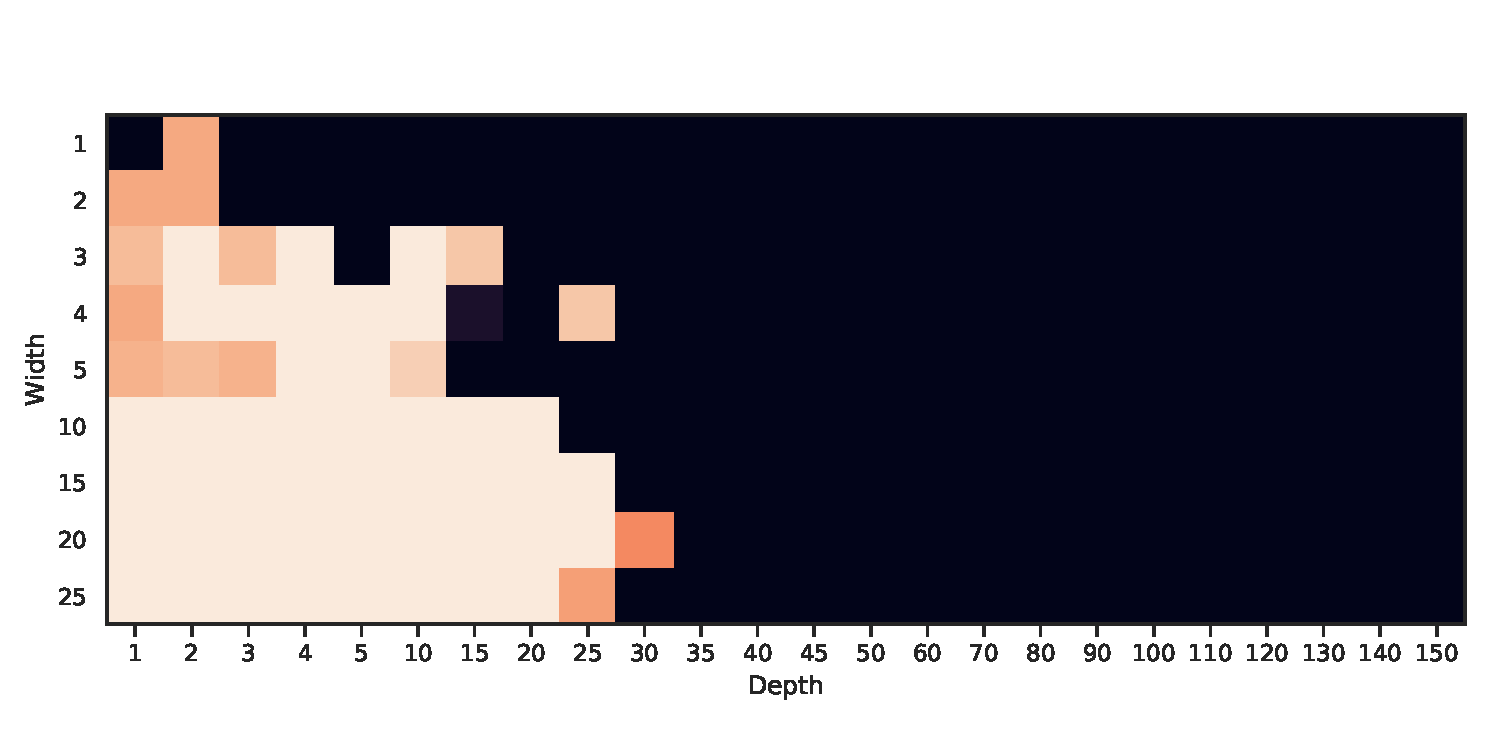
\includegraphics[width=\textwidth]{img/moons_grid/acc-relu.pdf}
        \caption{\ReLU training}
        \label{fig:moons_grid_relu}
    \end{subfigure}
    ~ %add desired spacing between images, e. g. ~, \quad, \qquad, \hfill etc. 
      %(or a blank line to force the subfigure onto a new line)
    \centering
    \begin{subfigure}[b]{0.3\textwidth}
        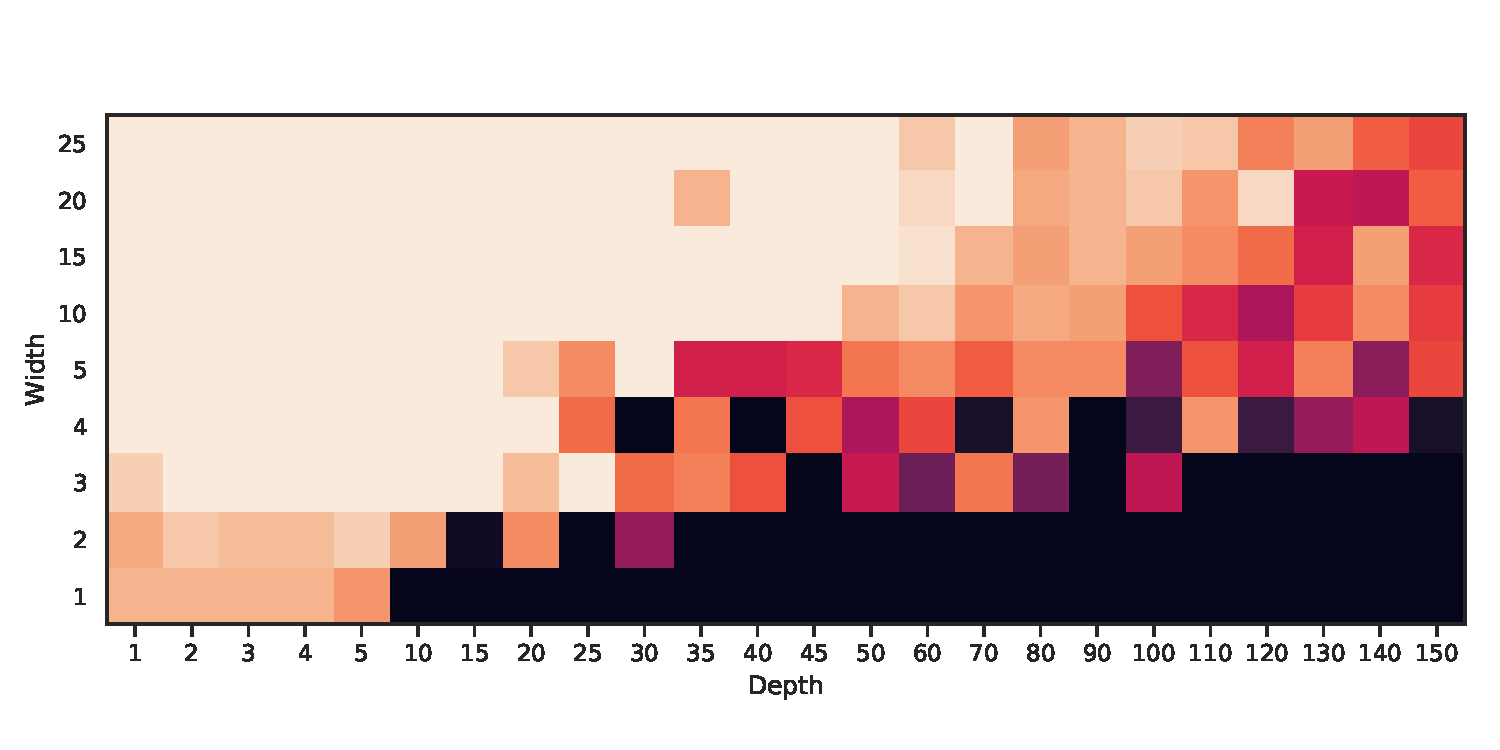
\includegraphics[width=\textwidth]{img/moons_grid/acc-relu-bn.pdf}
        \caption{\ReLUBN training}
        \label{fig:moons_grid_relubn}
    \end{subfigure}
    ~ %add desired spacing between images, e. g. ~, \quad, \qquad, \hfill etc. 
      %(or a blank line to force the subfigure onto a new line)
    \centering
    \begin{subfigure}[b]{0.3\textwidth}
        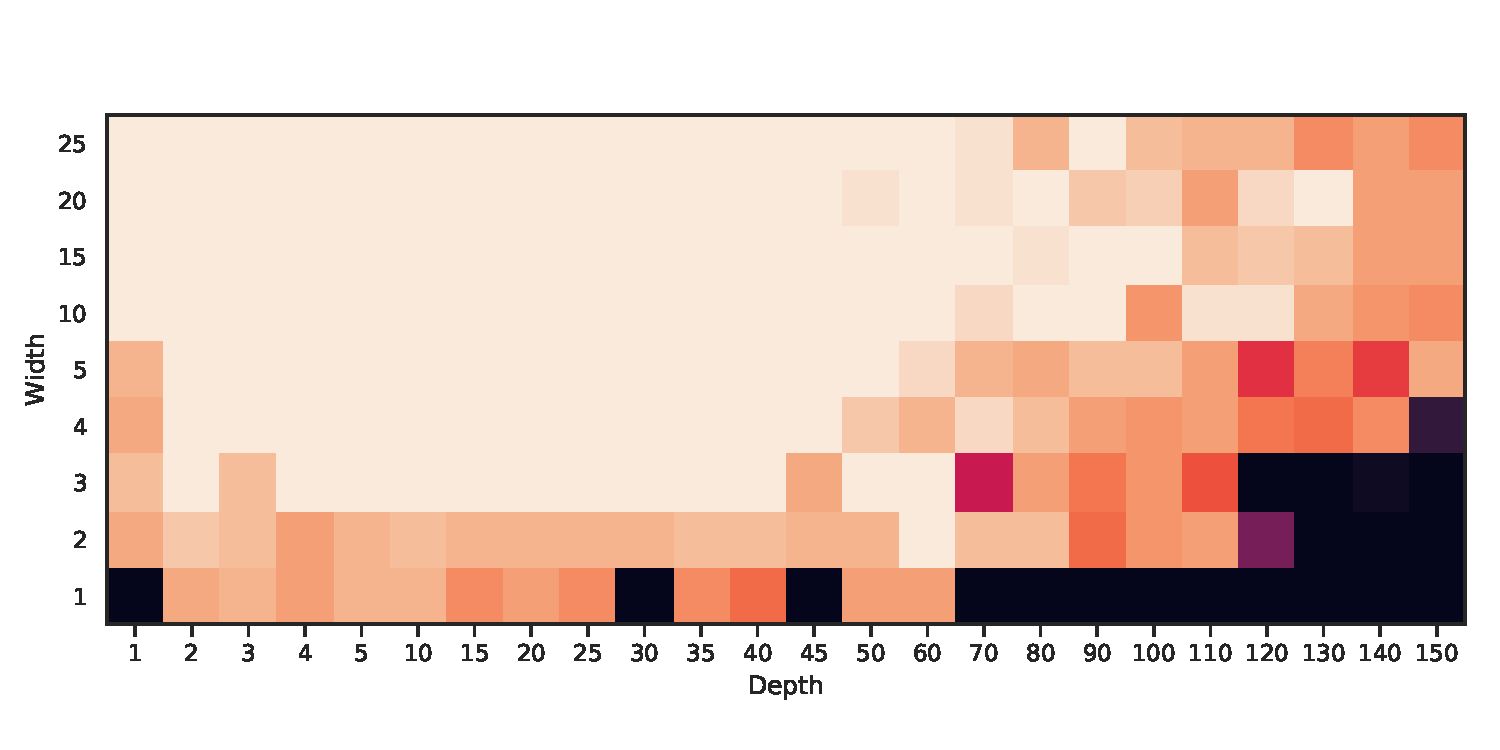
\includegraphics[width=\textwidth]{img/moons_grid/acc-sep-up-0-0001.pdf}
        \caption{\SepUnitPoint training}
        \label{fig:moons_grid_up}
    \end{subfigure}
    ~ %add desired spacing between images, e. g. ~, \quad, \qquad, \hfill etc. 
      %(or a blank line to force the subfigure onto a new line)
    \\
    \begin{subfigure}[b]{0.3\textwidth}
        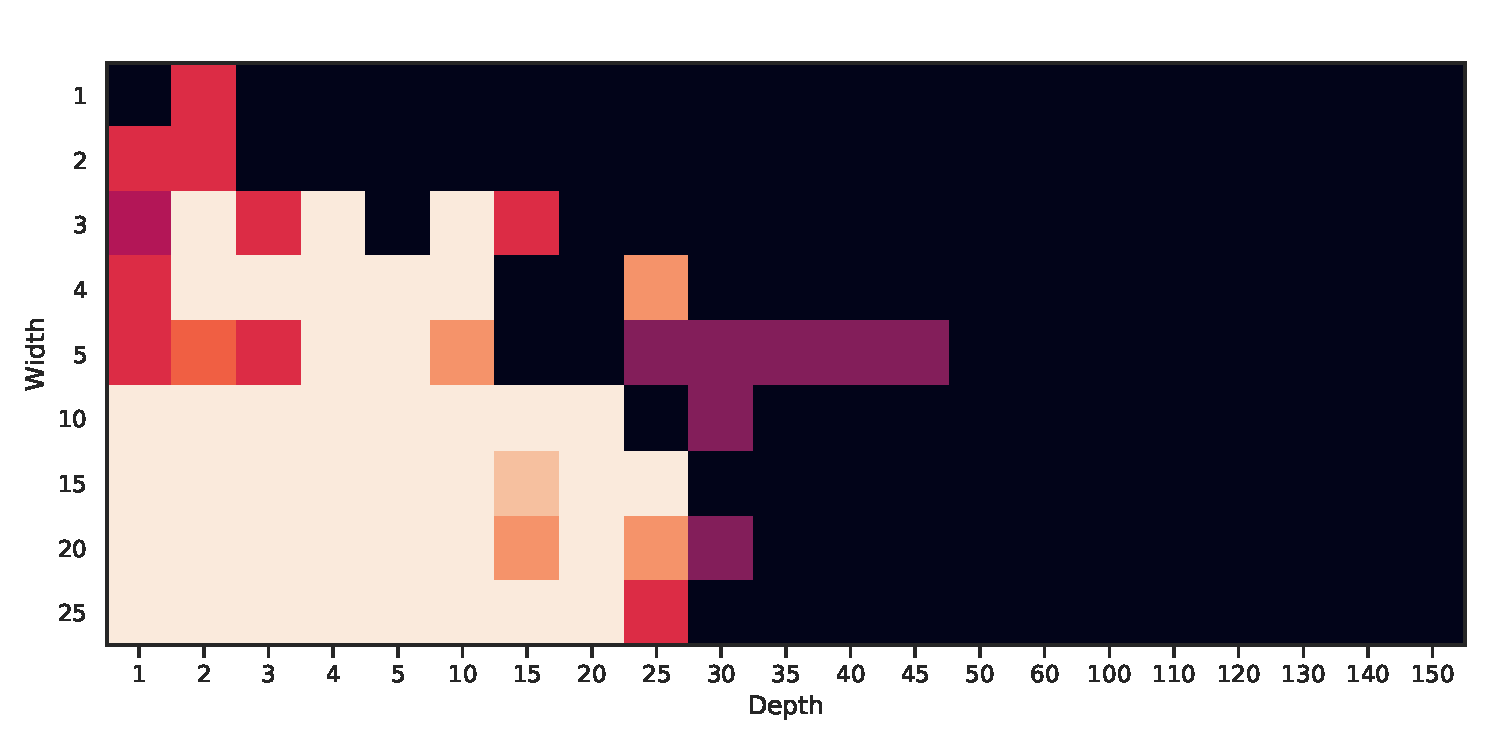
\includegraphics[width=\textwidth]{img/moons_grid/val-acc-relu.pdf}
        \caption{\ReLU validation}
        \label{fig:moons_grid_relu}
    \end{subfigure}
    ~ %add desired spacing between images, e. g. ~, \quad, \qquad, \hfill etc. 
      %(or a blank line to force the subfigure onto a new line)
    \centering
    \begin{subfigure}[b]{0.3\textwidth}
        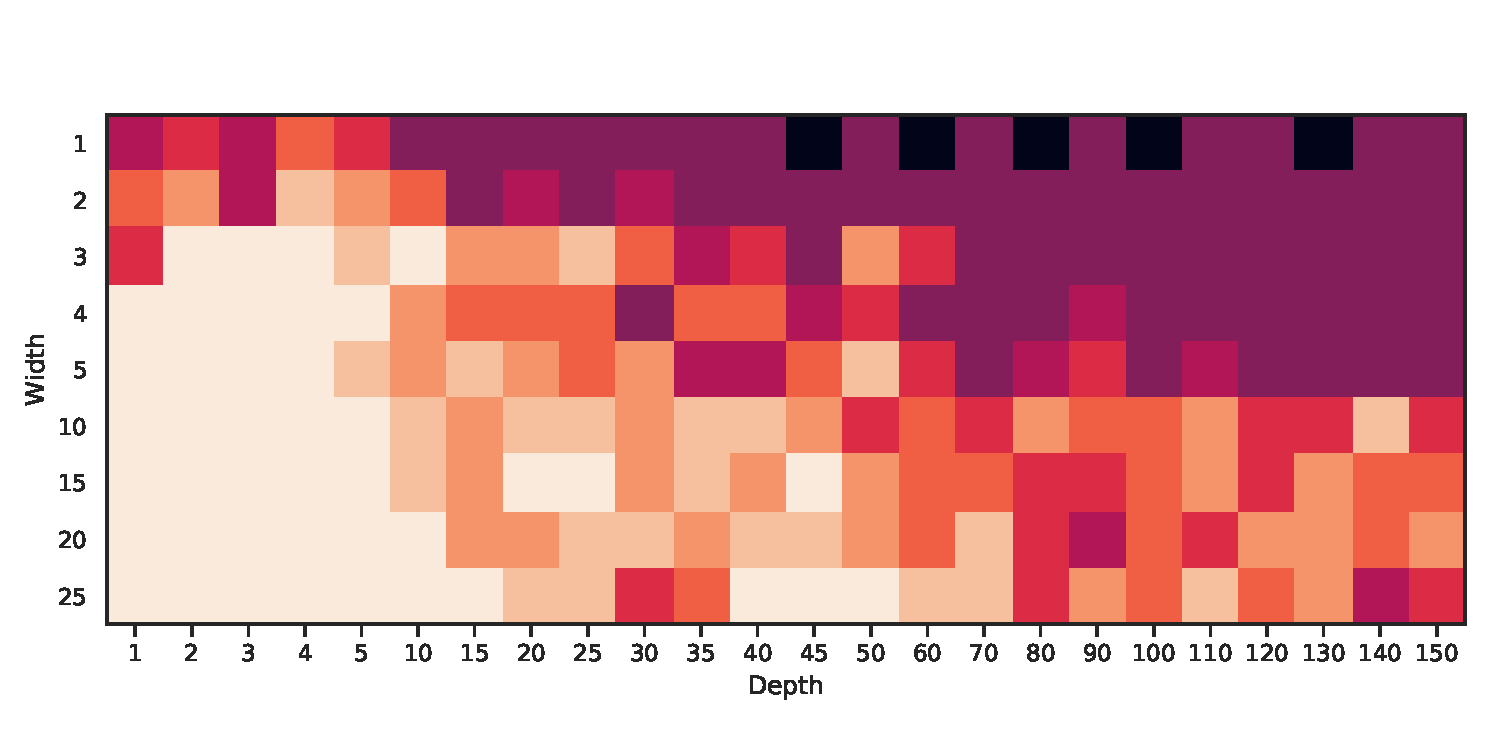
\includegraphics[width=\textwidth]{img/moons_grid/val-acc-relu-bn.pdf}
        \caption{\ReLUBN validation}
        \label{fig:moons_grid_relubn}
    \end{subfigure}
    ~ %add desired spacing between images, e. g. ~, \quad, \qquad, \hfill etc. 
      %(or a blank line to force the subfigure onto a new line)
    \centering
    \begin{subfigure}[b]{0.3\textwidth}
        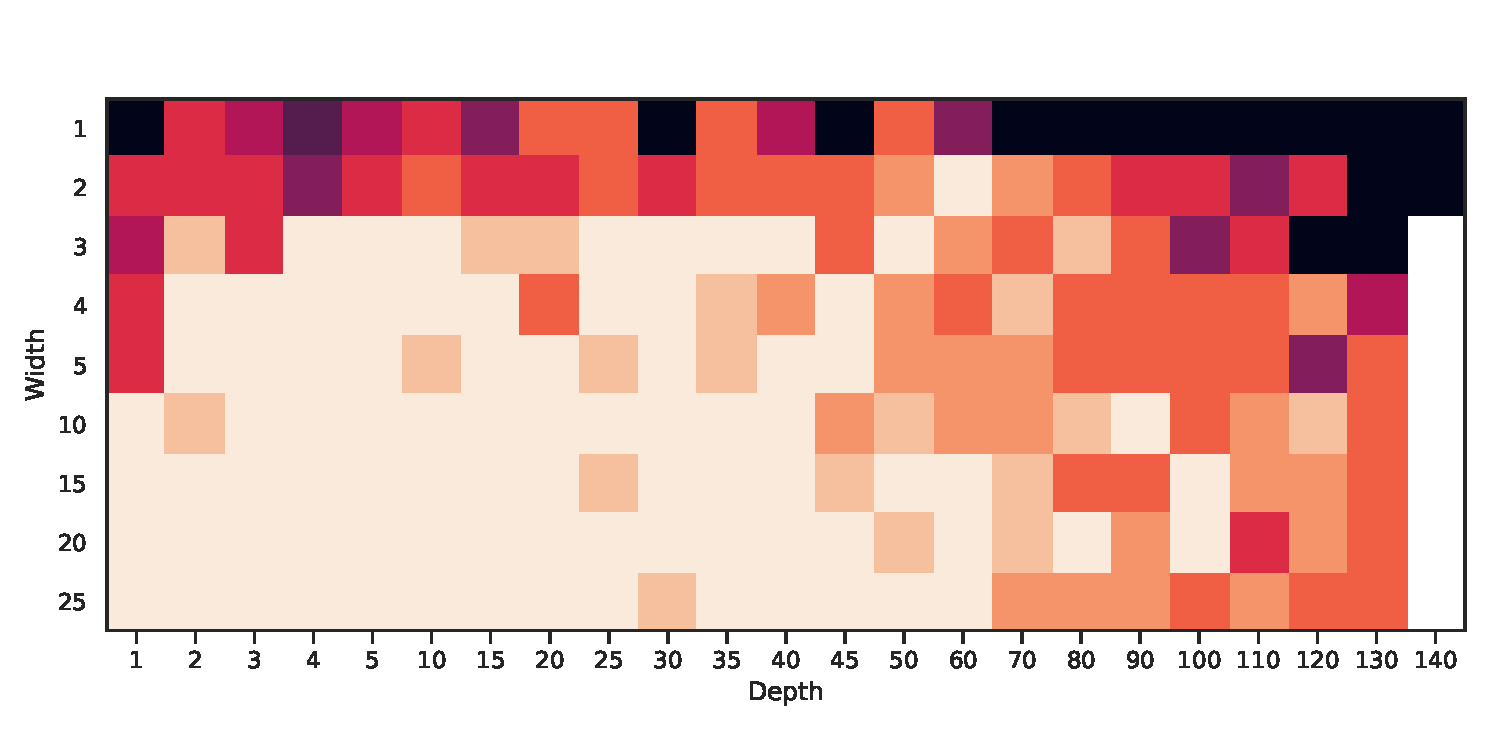
\includegraphics[width=\textwidth]{img/moons_grid/val-acc-sep-up-0-0001.pdf}
        \caption{\SepUnitPoint validation}
        \label{fig:moons_grid_up}
    \end{subfigure}
    ~ %add desired spacing between images, e. g. ~, \quad, \qquad, \hfill etc. 
      %(or a blank line to force the subfigure onto a new line)
      \\
    \begin{subfigure}[b]{0.3\textwidth}
        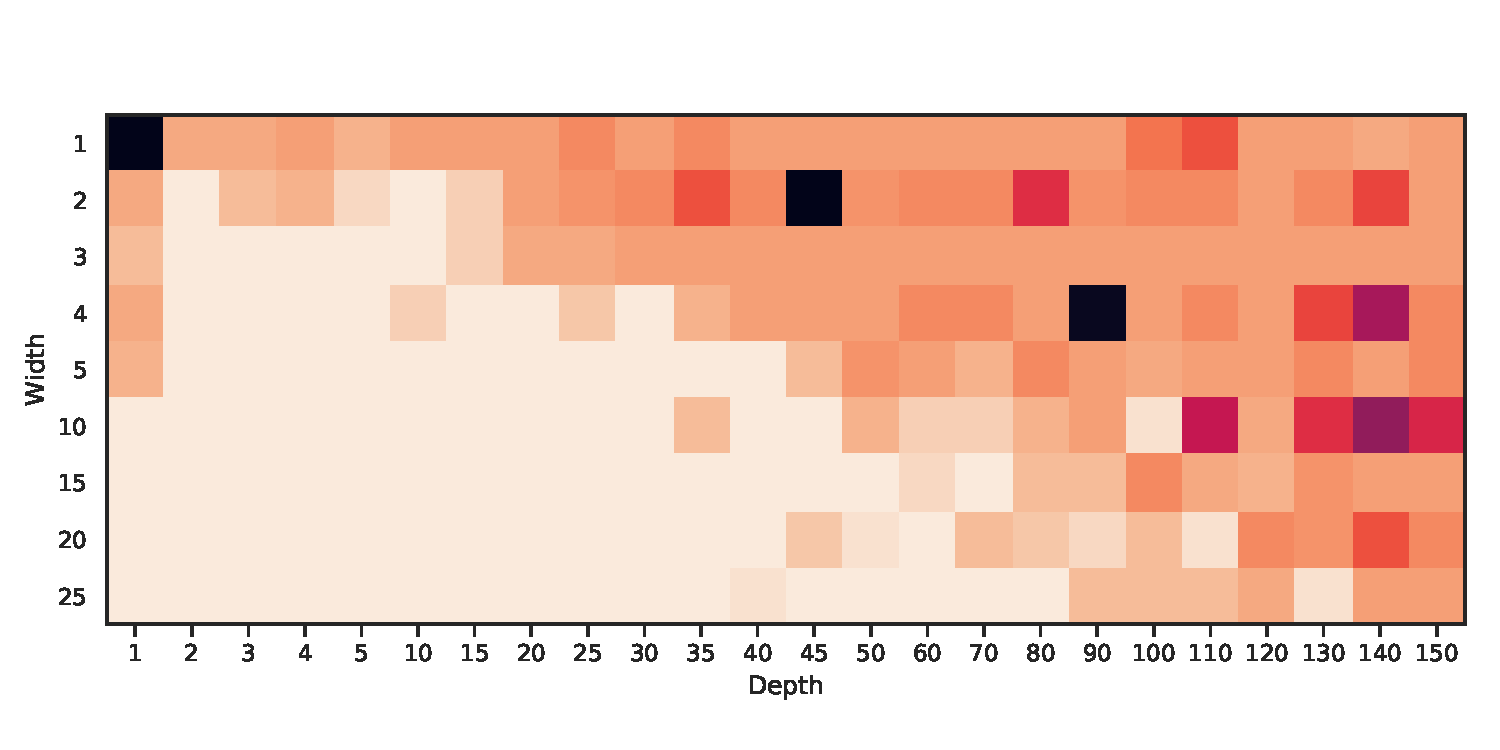
\includegraphics[width=\textwidth]{img/moons_grid/acc-sep-u-0-0001.pdf}
        \caption{\SepUnit training}
        \label{fig:moons_grid_u}
    \end{subfigure}
    ~ %add desired spacing between images, e. g. ~, \quad, \qquad, \hfill etc. 
      %(or a blank line to force the subfigure onto a new line)
    \centering
    \begin{subfigure}[b]{0.3\textwidth}
        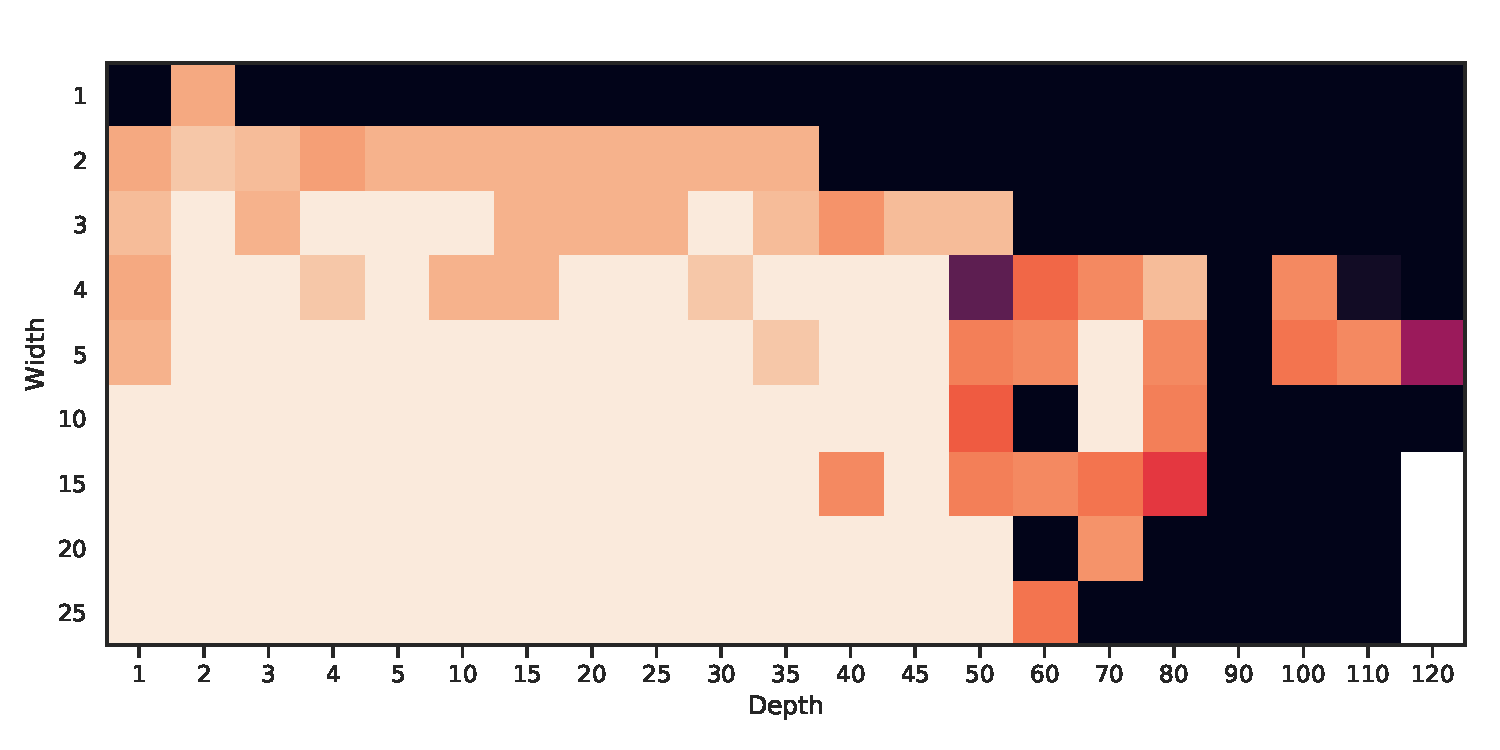
\includegraphics[width=\textwidth]{img/moons_grid/acc-sep-p-0-0001.pdf}
        \caption{\SepPoint training}
        \label{fig:moons_grid_p}
    \end{subfigure}
    ~ %add desired spacing between images, e. g. ~, \quad, \qquad, \hfill etc. 
      %(or a blank line to force the subfigure onto a new line)
    \\
    \begin{subfigure}[b]{0.3\textwidth}
        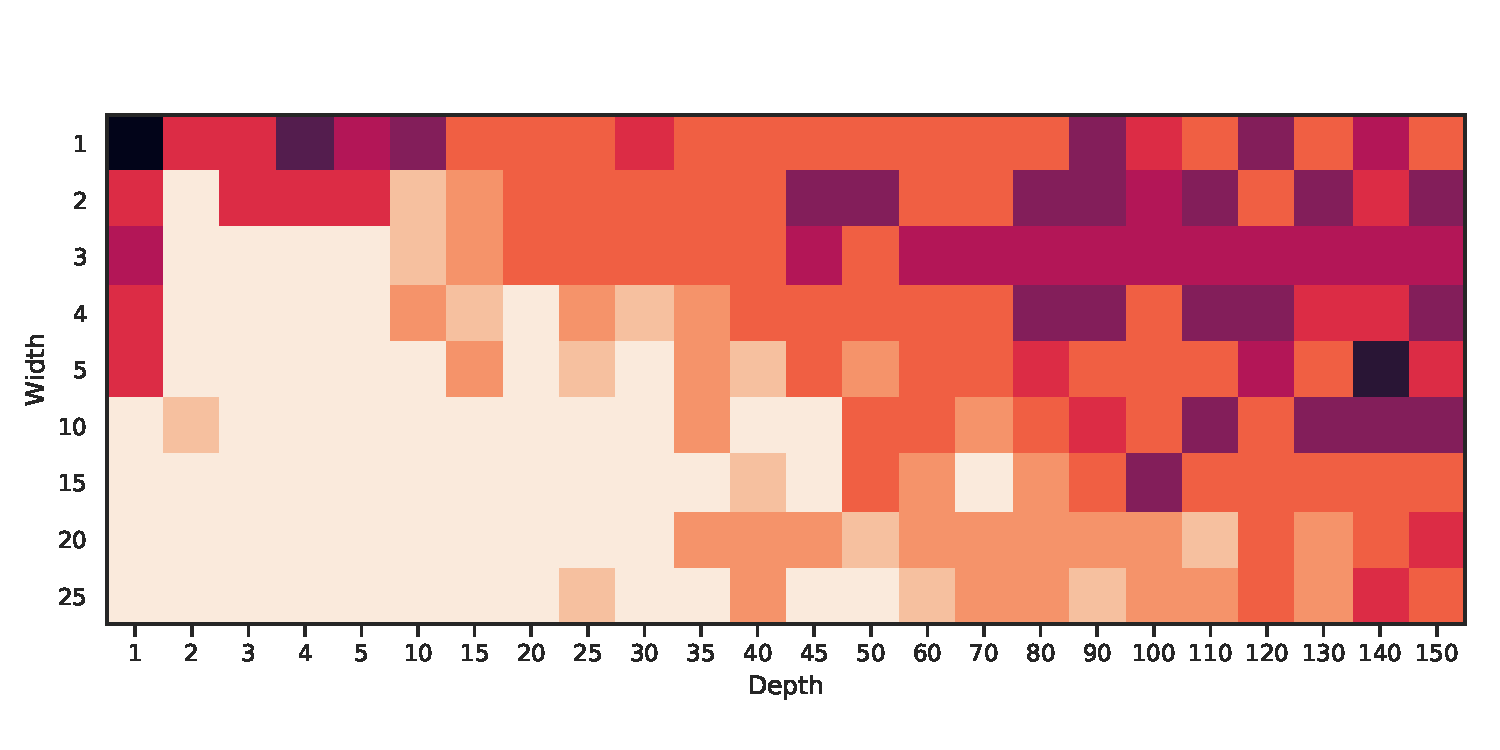
\includegraphics[width=\textwidth]{img/moons_grid/val-acc-sep-u-0-0001.pdf}
        \caption{\SepUnit validation}
        \label{fig:moons_grid_u}
    \end{subfigure}
    ~ %add desired spacing between images, e. g. ~, \quad, \qquad, \hfill etc. 
      %(or a blank line to force the subfigure onto a new line)
    \centering
    \begin{subfigure}[b]{0.3\textwidth}
        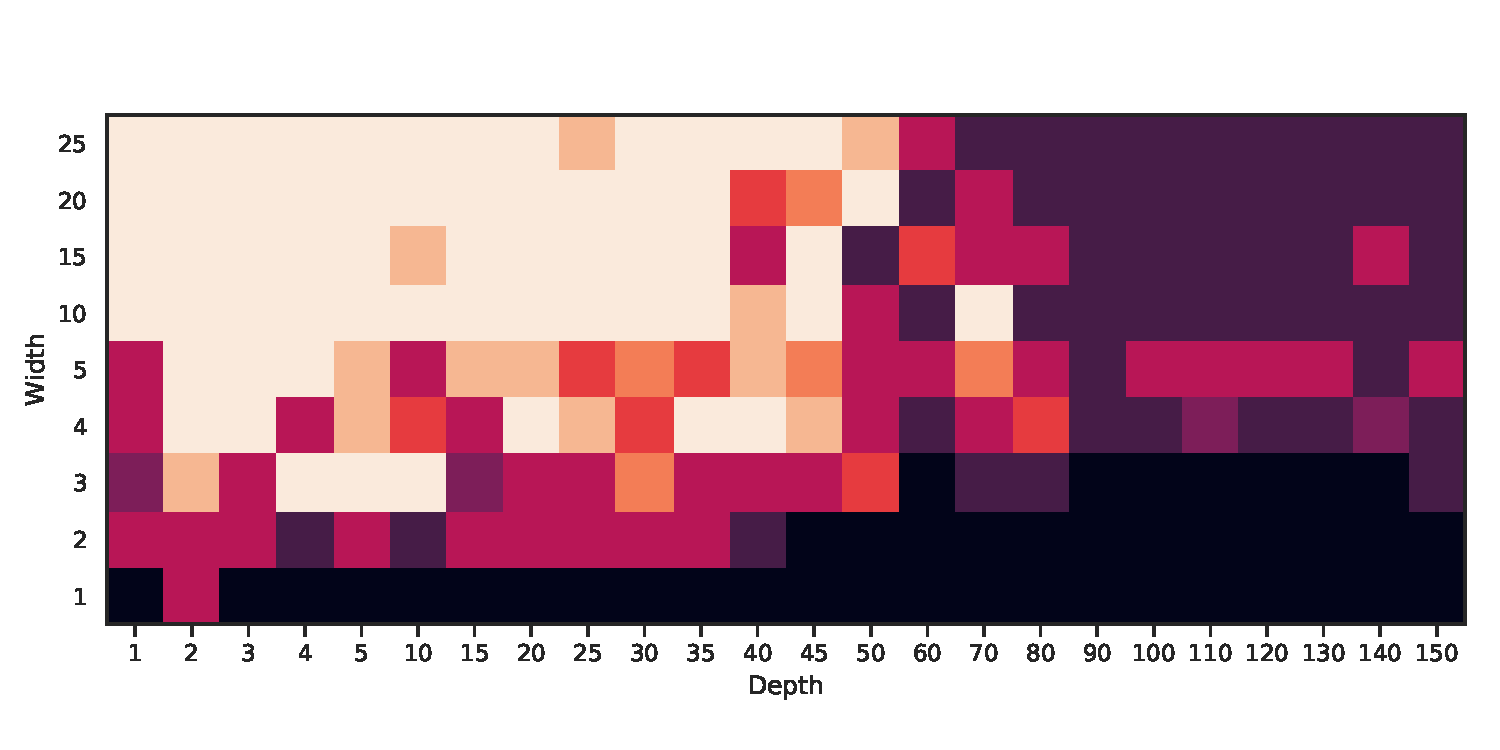
\includegraphics[width=\textwidth]{img/moons_grid/val-acc-sep-p-0-0001.pdf}
        \caption{\SepPoint validation}
        \label{fig:moons_grid_p}
    \end{subfigure}
    ~ %add desired spacing between images, e. g. ~, \quad, \qquad, \hfill etc. 
      %(or a blank line to force the subfigure onto a new line)
    
    
  \caption{Depth vs Width accuracy plot a for rectangular network using a grid (width from $2$ to $25$ and depth from $2$ to $150$),  trained using a Adam learning rate of $0.01$ in the \moons dataset. The color show the accuracy attained of each of the combinations of width and depth, the clearer the better. Notice how \ReLU, Figure \ref{fig:moons_grid_relu}, fails with networks deeper than 30 layers. In other hand, \ReLUBN, Figure \ref{fig:moons_grid_relubn}, manages to work until 70 layers deep. \SepUnitPoint,  Figure \ref{fig:moons_grid_up}, works significantly better than both, up to 120 layers. Notice how all the methods suffer from degradation from depth, which is partially alleviated by the use of greater width. This is consistent with \cite{simpnet} and \cite{densenet}. However, \SepUnitPoint is able to delay the apparition of the issue. This is especially visible when the number of units is small (from $2$ to $5$) where \ReLUBN fails to work whereas \SepUnitPoint does not. Regarding to the role of the constraint on its success, we find that \SepUnit, Figure \ref{fig:moons_grid_u}, allows the network to grow deeper, yet the accuracy can be lower following the linear decrease with the inverse of the width, which we blame on the inability of the \SepUnit constraint to address the \emph{dead point} issue. In the other hand, \SepPoint, Figure \ref{fig:moons_grid_p}, seems to perform well up to 50 layers, but it breaks down afterwards. Finally, \SepLayer , Figure \ref{fig:moons_grid_l} seems to suffer if the width is too large, performing well up to 70 layers.}
  \label{fig:moons_grid} 
\end{figure*}


\begin{figure*}
  \centering
    \begin{subfigure}[b]{0.3\textwidth}
        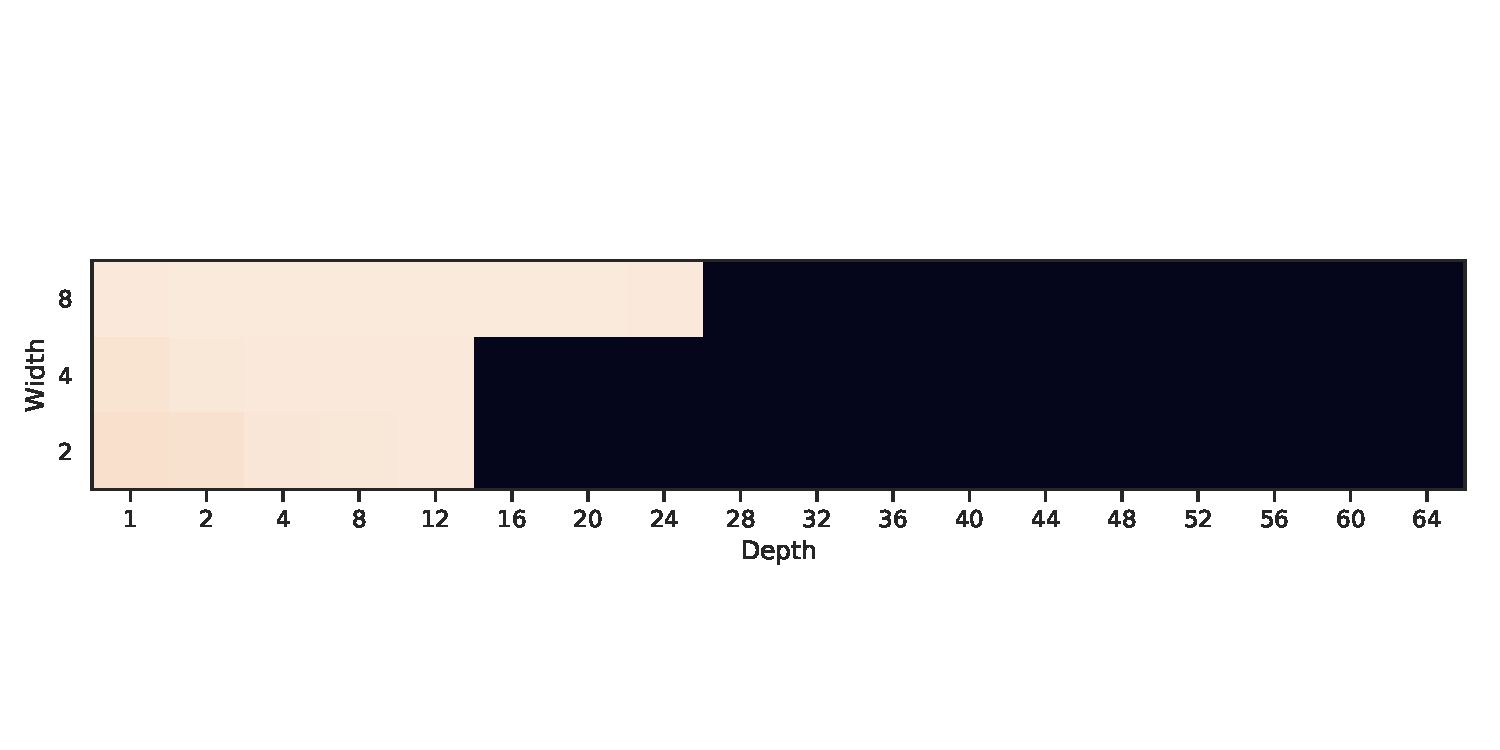
\includegraphics[width=\textwidth]{img/mnist_grid/acc-relu-ks-3x3-bs-1024.pdf}
        \caption{\ReLU}
        \label{fig:mnist_grid_relu}
    \end{subfigure}
    ~ %add desired spacing between images, e. g. ~, \quad, \qquad, \hfill etc. 
      %(or a blank line to force the subfigure onto a new line)
    \centering
    \begin{subfigure}[b]{0.3\textwidth}
        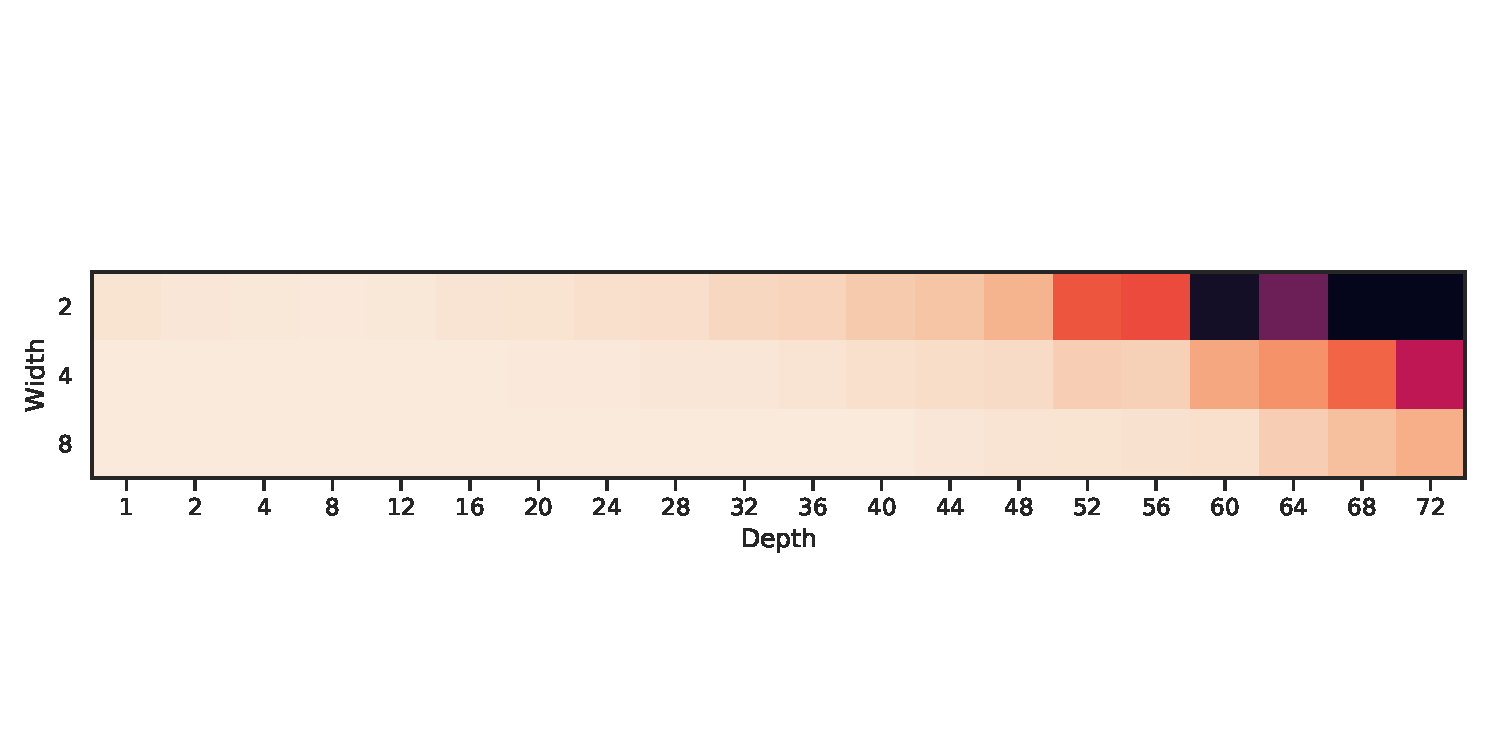
\includegraphics[width=\textwidth]{img/mnist_grid/acc-relu-bn-ks-3x3-bs-1024.pdf}
        \caption{\ReLUBN}
        \label{fig:mnist_grid_relubn}
    \end{subfigure}
    ~ %add desired spacing between images, e. g. ~, \quad, \qquad, \hfill etc. 
      %(or a blank line to force the subfigure onto a new line)
    \centering
    \begin{subfigure}[b]{0.3\textwidth}
        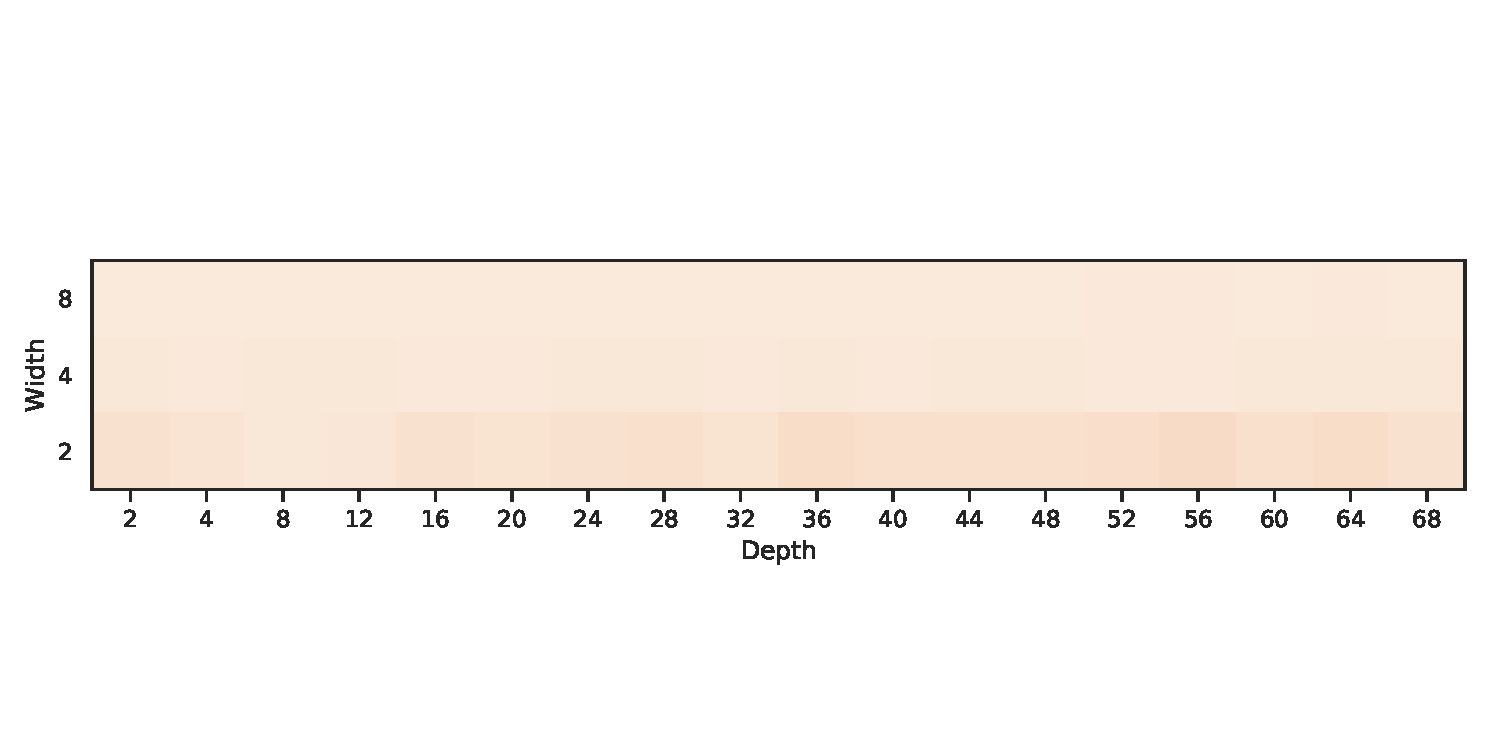
\includegraphics[width=\textwidth]{img/mnist_grid/acc-sep-up-1e-08-ks-3x3-bs-1024.pdf}
        \caption{\SepUnitPoint}
        \label{fig:mnist_grid_up}
    \end{subfigure}
    ~ %add desired spacing between images, e. g. ~, \quad, \qquad, \hfill etc. 
      %(or a blank line to force the subfigure onto a new line)
    
  \caption{Depth vs Width accuracy plot a for rectangular network using a grid (width from $2$ to $25$ and depth from $2$ to $150$),  trained using a Adam learning rate of $0.01$ in the MNIST dataset. The color show the accuracy attained of each of the combinations of width and depth, the clearer the better. Notice how \ReLU, Figure \ref{fig:mnist_grid_relu}, fails with networks deeper than 30 layers. In other hand, \ReLUBN, Figure \ref{fig:mnist_grid_relubn}, manages to work until 70 layers deep. \SepUnitPoint,  Figure \ref{fig:mnist_grid_up}, works significantly better than both, up to 120 layers. Notice how all the methods suffer from degradation from depth, which is partially alleviated by the use of greater width. This is consistent with \cite{simpnet} and \cite{densenet}. However, \SepUnitPoint is able to delay the apparition of the issue. This is especially visible when the number of units is small (from $2$ to $5$) where \ReLUBN fails to work whereas \SepUnitPoint does not.}
  \label{fig:mnist_grid} 
\end{figure*}



\begin{table*}
\begin{tabular}{llrrrrr}
\toprule
                    &    &       2  &       10 &       25 &       30 &       40 \\
\midrule
relu ks 3x3 & 10 &  0.72142 &  0.82748 &  0.09906 &  0.09880 &  0.09810 \\
relu-bn ks 3x3 & 10 &  0.90580 &  0.81764 &  0.70496 &  0.66718 &  0.59642 \\
Sep-UP 1e-08 ks 3x3 & 10 &  0.69264 &  0.79044 &  0.74344 &  0.70452 &  0.68416 \\
\bottomrule
\end{tabular}

\\
\begin{tabular}{llrrrrr}
\toprule
                    &    &      2  &      10 &      25 &      30 &      40 \\
\midrule
relu ks 3x3 & 10 &  0.5958 &  0.6052 &  0.1000 &  0.1000 &  0.1000 \\
relu-bn ks 3x3 & 10 &  0.5682 &  0.5385 &  0.5414 &  0.5328 &  0.4512 \\
Sep-UP 1e-08 ks 3x3 & 10 &  0.5874 &  0.5703 &  0.5353 &  0.5300 &  0.5320 \\
\bottomrule
\end{tabular}

\caption{}\label{tab:cifar10}
\end{table*}
\section{Conclusions}\label{sec:conclusions}

% PREGUNTA DEL PAPER
% Since the existing methods require either computational expenditure and add arbitrary complexity to the architecture design, or simply entail limit network performance, we wonder whether we can train deeper networks without relying in any of those techniques. This imply using the minimum width possible, removing any additional connections or activations, and using no normalization. 

% 1.1
The separation constraint is \emph{comparable} to the usual techniques (as presented in the introduction). Indeed, \SepLayer allows for affine units (recall Equation \ref{eq:affineUnit}) that forward representations between layers in the same spirit as ResNets \cite{resnet} or DenseNets \cite{densenet}. Meanwhile, a layer satisfying the \SepPoint constraint ensures the existence of two units with opposite-facing hyperplanes similarly to \texttt{C-ReLU} \cite{crelu}. In addition, the intuition of the separation constraint method intends to serve as stronger heuristic for parameter configuration (independently of initial values), so that units reach a useful configuration for backpropagation, instead of insisting on reaching on some \emph{favorable} initial configuration via trial-and-error as done in the layer-width-increase approach \cite{wideresnet,inceptionv1}.   
\\\\
% 2.1
We claim that there is a difference between non-zero and \emph{useful} activations. As presented in Figure \ref{fig:moonsReLUBN}, \ReLUBN induces a solution that maps the dataset non-trivially throughout the network. However, its performance on the \texttt{MOONS} dataset is inferior to our proposal (63\% of accuracy as presented in Table \ref{tab:moons} against any constraint based test over 90\%). Moreover, comparing the output graph of \ReLUBN (Figure \ref{fig:moonsReLUBNOutput}) with our findings (Figures \ref{fig:moonsUnitwiseOutput}, \ref{fig:moonsPointwiseOutput}. \ref{fig:moonsLayerwiseOutput} and \ref{fig:moonsUnitpointwiseOutput}) the reader can observe that the separation reached separates components of the \texttt{MOONS} dataset in intuitive manners.  
\\\\
% 3.1
The separation constraints compels the data to go through the network favorably for the cross-entropy loss back-propagation. Experimentally, Figure \ref{fig:peaks} suggests that the training phase begins with minimizing the constraint loss until a certain level (approximately $0.21$ around epoch 750), enabling the optimization of the main loss (recall 80 to 100\% accuracy in our tests in Table \ref{tab:moons}). Analytically, we can elaborate on this behavior if we are reminded of the fact that the gradient of the main loss is non-zero \emph{on} the upper sets of units by virtue of Equation \ref{eq:upperPartOfUnit} and the separability conditions presented in subsection \ref{subsec:ReLUSeparability}. Thus, ensuring non-empty upper sets of units is a sufficient condition for back-propagation. 
\\\\
However, further inquiry into the interaction between constraint loss and main loss beyond parameter $\lambda$ is needed. Anecdotal evidence shows spurious transient states on convergence in the cases of \SepPoint, \SepUnit and \SepUnitPoint, but not on \SepLayer.  Additionally, in the scope of our experimentation we have chosen the cross-entropy loss functional, further inquiry is required on the choice of main loss. Another topic that demands further investigation is the use of the separation constraints in other types of layers such as convolutional \cite{lenet}, LSTM \cite{lstm} or transformers \cite{transformer}\cite{transformer2}; other types of tasks such as regression, unsupervised learning, \cite{embedding} graph \cite{graph} or generation \cite{gan}\cite{vae}; and especially more challenging datasets.
\\\\
% 4.1
While the separation constraints prevent the vanishing gradient, the \emph{exploding gradient} remains at large. Notice that the constraints designed place \emph{lower bounds} on the magnitude of the pre-activation values, it places no upper bound. Analytically, this gradient depends on both on the magnitude of the weight vectors, absolute value of the biases and  the magnitude of dataset points mapped throughout the network. This could be solved introducing additional constraints or limiting the norms of weight vectors. 
\\\\
Despite the fact that we intended to avoid dead and affine neurons with our geometrical formulation (recall the predicate $R_1(u) \wedge R_2(u)$ defined on Equation XXX) the different constraints  object in practice. While $R_1(u) \wedge R_2(u)$ is valid within \SepUnit and from it, it extends to layers, \SepLayer and \SepPoint,  allow at least on unit to be affine  over the dataset (recall Equation \ref{eq:affineUnit}) and at least another to be dead (recall Equation \ref{eq:deadNeuronVersion2}), invalidating $R_1(u) \wedge R_2(u)$ for each unit in a layer $\layer$, but holding $R_1(\layer) \wedge R_2(\layer)$. 
\\\\
In this sense, neither \emph{repeated} (producing the same upper set), affine nor dead units are \emph{harmful} for network performance, beyond burdening networks with additional non used parameters. They seem ubiquitous in the extent of our experimentation as Figures \ref{fig:moonsLayerwise}, \ref{fig:moonsPointwise} and \ref{fig:moonsUnitpointwise} testify (see the axis-aligned or diagonally expanding intermediate representations of the dataset). Further inquiry is needed to understand how dead, affine and repeated neurons coalesce in solving the problem. In addition, our experimentation suggests that the  the distribution of dead, affine and repeated units varies according to constraint type (in the extent of our experimentation). 
\\\\
Indeed, Figure \ref{fig:moonsLayerwise} for the \SepLayer constraint type showcases a feature layer (divisions \ref{fig:moonsLayerwiseFeature1} and \ref{fig:moonsLayerwiseFeature1}) with two dead units and two repeated. Meanwhile Figure \ref{fig:moonsUnitwise} at the 24th layer (divisions \ref{fig:moonsUnitwise251} and \ref{fig:moonsUnitwise252}), depicts repeated neurons (organized pairwise) with no affine nor dead units. 
\\\\
Analytically, we can approach affine units in the same spirit as \texttt{ResNet} \cite{resnet} or \texttt{DenseNet}\cite{densenet}. Since the composition of affine functions is affine, collections of successive (across the layers) affine units effectively \emph{shortcut} the network. Experimentally, we verify this in our \SepLayer experiments (as it is the only separation constraint that allows affine units). Notice that there is a coalescence between axis-aligned and diagonal units that preserves the topology of the intermediate representation of the dataset after layer 4, see Figures \ref{fig:moonsLayerwise42} and \ref{fig:moonsLayerwiseFeature2} are almost equal. We conjecture that repeated units perform the same role for \SepUnit, since affine units are forbidden with this constraint. Notice how in Figure \ref{fig:moonsUnitwise252} all the planes are cutting at the same point, thus having the same \emph{upper} and \emph{lower} sets. Interestingly, those sets are compressed into two points in the feature layer (Figures \ref{fig:moonsUnitwiseFeature1} and \ref{fig:moonsUnitwiseFeature2}), but if we add \SepPoint as in \SepUnitPoint we find the same behaviour again, where the feature layer is similar to the inner representation at layer 25 (Figures \ref{fig:moonsUnitpointwise252} and \ref{fig:moonsUnitpointwiseFeature2}). 
\\\\
We explore the use of separation constraint (\SepUnitPoint in this case) to enable zero initialization with good results, see Section \ref{subsec:zero}. In order to make it work though, we had to introduce  means to break the symmetry between the positive and negative constraint ,in the form of $\rho$ (see Equation \ref{eq:definitionOfRho}), and to break symmetry in the weights, in the form of Annealed Dropout \cite{dropoutAnnealing}. Since our objective in this matter (along with all the paper) was simplicity, and the use of Dropout partially defeats this purpose by moving the same stochasticity that we were removing from intialization into training. Nevertheless, our \emph{ansatz} is that an initialization that is based on the data (which is the result of using the constriant plus Dropout) must be superior to any random initialization which is only based in features like gradient magnitude or inputs and outputs. Further research in this matter is hereby required.









%%%%%%%%%%%%%%%%%%%%%%%%%%%%%%%%%%%%%%%% BIBLIOGRAPHY %%%%%%%%%%%%%%%%%%%%%%%%%%%%%%%%%%%%%%%%%%%%%%%%%%%%%%%%%%%%%%%%%
{\small
\bibliographystyle{ieee}
\bibliography{references}
\nocite{*}
}

\end{document}

